\documentclass{article} % For LaTeX2e
\usepackage{times}
\usepackage{hyperref}
\usepackage{url}
\usepackage{cite}
\usepackage{times}
\usepackage{tikz}
\usetikzlibrary{arrows,decorations.pathmorphing,fit,positioning}
\usepackage{algorithmic}
\usepackage{mdframed}
\usepackage[margin=1in]{geometry}
\usepackage{amsmath}
%\documentstyle[nips14submit_09,times,art10]{article} % For LaTeX 2.09


\title{Topic extraction for music genre using lyrical content}


\author{
Sharon Gieske \\
\texttt{6167667}\\
\texttt{sharongieske@gmail.com} \\
\and
David van Erkelens\\
\texttt{10264019}\\
\texttt{daviddvanerkelens@gmail.com} \\
\and
Elise Koster \\
\texttt{5982448}\\
\texttt{koster.elise@gmail.com}
}


% The \author macro works with any number of authors. There are two commands
% used to separate the names and addresses of multiple authors: \And and \AND.
%
% Using \And between authors leaves it to \LaTeX{} to determine where to break
% the lines. Using \AND forces a linebreak at that point. So, if \LaTeX{}
% puts 3 of 4 authors names on the first line, and the last on the second
% line, try using \AND instead of \And before the third author name.

\newcommand{\fix}{\marginpar{FIX}}
\newcommand{\new}{\marginpar{NEW}}

%\nipsfinalcopy % Uncomment for camera-ready version

\begin{document}


\maketitle

\begin{abstract}
%1 paragraph: main idea and a key finding \\
Genre classification and music recommendations are an important service of online music providers. Since manual genre classification is very time-consuming, especially with ever larger quantities of music available, an accurate classifier for music genres enhances the user experience of music providers and provides insight into themes that differentiate genres from each other. This paper proposes an extension of LDA to model topics over genres instead of documents, and shows that this extension outperforms regular LDA on classification tasks.
\end{abstract}
\clearpage
\section{Introduction}
max 2 pages:
\begin{itemize}
\item Description of problem area and problem itself
\item What is the research question/goal?
\item Why is this is an important/meaningful/interesting problem to consider?
\item the very basic idea of the approach and why is this a reasonable approach for this problem?
\end{itemize}

	\subsection{Background}
Music genre classification has been researched mostly using audio signals. While this approach uses the \textit{defining} characteristic of music, namely, its musical structure, an other interesting approach is to use word-based analysis.

\section{Problem}
roughly 1-2 pages
\begin{itemize}
\item explain the problem; what kind of assumptions/observations you have about the problem
\end{itemize}

\section{Approach}
For this research the following framework is used:
\begin{enumerate}
	\item Gather dataset using crawler
	\item Preprocessing (removal of stop words etc)
	\item Model topics and extract topic distribution for documents
	\item Train SVM on array of topic-probabilities per document (and its genre)
	\item Generate `song' of length $n$ for genre $g$: select topic $k \sim \theta_g$ then select word $w \sim \varphi_k$, repeat $n$ times
\end{enumerate}

In the following subsections the dataset is described in section \ref{sub:prep} and the extended LDA model is explained in section \ref{sub:ext-lda}. The classification and evaluation methods are described in section\ref{sub:classification} and the method to generate a song is displayed in section \ref{sub:song}

\subsection{Data acquisition}\label{sub:prep}
Before any model could be tested, data had to be collected and processed. To do this, a crawler was built that collects song lyrics from \textit{Lyricsmode}\footnote{\texttt{http://www.lyricsmode.com}} by going through the alphabet (with one `letter' for numbers $0-9$), finding the top 100 artists starting with that letter and collecting the first five songs (alphabetically) by that artist. After collecting these lyrics, genre-information was retrieved from \textit{Allmusic}\footnote{\texttt{http://www.allmusic.com}}. The choice of these websites are primarily based on earlier research \cite{felllyrics} that used these websites because of their consistency. \\
After collecting a dataset of $12.102$ lyrics, the data was pre-processed to filter out \textit{a)} punctuation marks and capitalization \textit{b)} non-english lyrics and \textit{c)} low-content, very common words\footnote{For example, 'a', 'by', 'I', 'off', 'were'}, resulting in a dataset of $9.728$ lyrics. These pre-processing steps were done under the assumption that for topic modeling, including common words would create low-information topics that would hardly contribute to the model. Another assumption was made that punctuation and capitalization, while containing useful information regarding language, were not relevant to the kinds of topics that would be found (as topic modeling is usually a bag-of-words approach). Non-english lyrics were filtered because extraction topics over multiple language would add a lot of noise to the model. Note however, that not \textit{all} non-english words were filtered out (only complete songs in a different language): in many cases, the use of \textit{some} non-english words can say a lot about a genre\footnote{Think of the Latin genre, for example, which turned out to use both english and spanish words quite a lot}. 

\subsection{Extended LDA model}\label{sub:ext-lda}
Latent Dirichlet Allocation (LDA) treats every document like a collection of words, and presumes that each word in a document is generated by a certain topic. A hidden distribution over topics is assumed to exist for every document. The goal of LDA is to \textit{a)} find a distribution over topics for each document and \textit{b)} find a distribution over words for each topic. Thus, we're looking for two sets of distributions: $\theta_i \sim \text{Dirichlet}(\alpha)$, or a distribution of topics over document $i$, and $\varphi_k \sim \text{Dirichlet}(\beta)$, or a distribution of words over topic $k$. Thus, LDA assumes that some generative model generates a document: for each word position $i,j$ from $i \in$ documents and $j \in$ words$_i$, choose a topic $z_{ij} \sim \theta_i$, then choose a word $w_{ij} \sim \varphi_{z_{ij}}$. \\
In this paper, LDA is extended: instead of finding distributions over topics for every document, topic distributions are learned over genres, where a genre is a non-overlapping set of documents. The difference between regular LDA and genre-LDA can be seen in the graphical models found in figure \ref{fig:graphical-model} (original LDA) and \ref{fig:graphical-model_extended} (genre-LDA). \\
To infer the different distributions, collapsed Gibbs sampling is used (where the distributions $\theta_i$ and $\varphi_k$ are integrated out). The derivation for genre-LDA is similar to, but not exactly the same as the derivation for original LDA. The derivation as well as the symbol description can be found in section \ref{ref:derivation}.\\

\begin{figure}[htp]
	\centering
	\begin{subfigure}[b]{0.5\textwidth}
		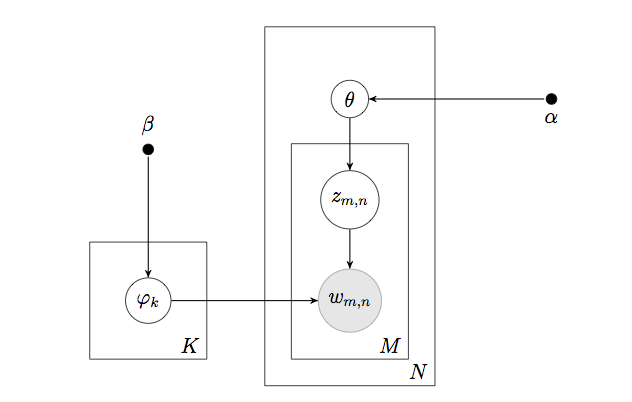
\includegraphics[width=\textwidth]{regular_lda_img}
		\caption{Graphical model for regular LDA}
		\label{fig:graphical-model}
	\end{subfigure}%
        \begin{subfigure}[b]{0.5\textwidth}
		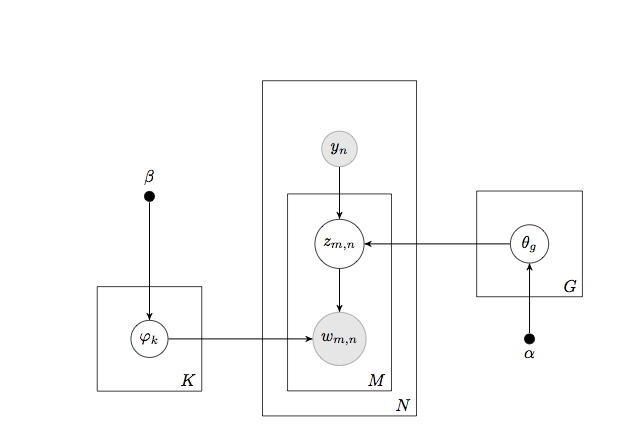
\includegraphics[width=\textwidth]{extended_lda_img}
		\caption{Graphical model for extended LDA}
		\label{fig:graphical-model_extended}
	\end{subfigure}
\end{figure}



\subsubsection{Gibbs sampling}
The calculation of the total probability of the model is computationally difficult because it marginalizes by integrating over a joint distribution. Therefore, the collapsed Gibbs sampling algorithm is applied for the (extended) LDA model. This algorithm samples from a conditional distribution which asymptotically approaches the correct distributions and is computationally simple compared to the marginalization of the total probability. The formula for the conditional probability used in Gibbs sampling algorithm for the extended LDA model can be found in section \ref{ref:derivation}. As can be seen in this formula, the conditional probability is also dependent on the counts of topics that occur in documents with the same genre instead of only the document in question.

\begin{mdframed}
\begin{algorithm}[H]\label{alg:create-song}
 \KwData{Topic Model inferred by extended DA, genre $G$, number of documents $N$, words in document i $M_i$}
 \KwResult{word-topic and topic-genre distribution}
\textbf{Initialize:} randomly assign words to topics \\
 assign topics to genre given genre of doc in which word is found\\
 \For{ Document $i$ where $i\in 1\dots N$ }{
 	\For{word $j$ where $j\in 1\dots M_i$}{
  calculate conditional probability distribution for $z_{i,j}$\\
  sample topic from distribution $k$\\
  update word-topic distrubtion given $z_{ij} = k$\\
  update topic-genre distrubtion given $G$\\
	}
 }
 return word-topic distribution, topic-genre distribution
 \caption{Gibbs sampling for extended LDA}
\end{algorithm}
\end{mdframed}

\subsection{Classification}\label{sub:classification}
In order to classify documents into their genres, a multi-class Support Vector Machine (SVM) classifier is implemented with the use of python module Scikit-Learn\cite{scikit-learn}. The SVM classification is a state-of-the-art classification algorithm for supervised learning which constructs a hyper-plane in high dimensional spaces with largest distance to the nearest training data points of any class. In this research a multi-class SVM is used which incorporates a One-vs-All strategy where it fits one classifier for each class.

As input the topic distribution for each document in the training set is calculated and their class (i.e. genre) is given to the multi-class SVM to train the classifiers. Then the classifier predicts the genres for the test set given their topic distribution for each document. With the use of the F1-score (section \ref{sub:f1}) the predictions of the classifier are evaluated.

\subsubsection{F1-score}\label{sub:f1}
The classifications are scored with the use of the F1-score. The F1-score is a measure which takes into account the precision and recall scores of the model and can be seen as a weighted average. The precision score takes into account the number of true positives divided by the true and false positive documents that are retrieved. The recall score takes into account the number of number of true positives divided by the total positive documents that should have been retrieved. The calculation of the F1 score is displayed below.

\begin{align}
F1 = 2 * \frac{precision * recall }{precision + recall}
\end{align}


\subsection{Generative model}\label{sub:song}
Since LDA is a generative model, it can also be used to create new lyrics. To create a `song' of length $n$ for a genre $G$, for each word position from $0$ to $n$, a topic $k$ is sampled from $G$'s topic distribution. Then, a word is sampled from $k$'s word distribution (see also algorithm \ref{alg:create-song}). \\
\begin{mdframed}
\begin{algorithm}[H]\label{alg:create-song}
 \KwData{Topic Model inferred by extended LDA, genre $G$, length $n$}
 \KwResult{Song for genre $G$ of length $n$}
 initialize: song = `' \\
 \While{counter $< n$ }{
  sample $k \sim \theta_G$\\
  sample $w \sim \varphi_k$\\
  append $w$ to song\\
  counter ++ \
 }
 return song
 \caption{Song generation}
\end{algorithm}
\end{mdframed}



\section{Experiments/Empirical Evaluation}
roughly 2-3 pages
\begin{itemize}
\item any details about experiments (dataset sizes, parameter selection, etc)
\item results
\item analysis (discussion of results/visualizations/findings/etc)
\end{itemize}


\section{Discussion and Conclusions}
\subsection{Challenges}
One of the main challenges of the research was caused by the dataset: the dataset consists for a large part of \verb|pop/rock| songs, in which both easy-to-listen top 40 songs are included, but also death metal songs. The diversity of this genre makes it quite hard to classify, since such a broad genre contains a lot of different words and therefore a pretty even distribution over topics. \\
Another challenge faced was the fact that some words, like \textit{love} occur in a lot of different genres. Words that occur in a lot of different genres make it harder to have a topic distribution with a high probabilty for only a couple of topics and should therefore be filtered from the dataset. 

\subsection{Conclusion}
It can be concluded that the extended version of LDA forms sensible topics for different genres, especially the genres named after their content. However, due to the very uneven distribution of lyrics over genres, it became hard to classify the test set and reach a high F1 score. The extended version of LDA did perform better than regular LDA, which is a sign that extended LDA with Gibbs sampling is a sensible choice to form topics based upon genres. \\
Using a SVM with the topic distributions over genres, an average correct prediction was given in about 57\% of the lyrics in the test set. Using a better distributed data set with more distinct genres, this number should increase. Still, the performance of the algorithm was way better than the performance of a baseline classifier, which predicted no more than 42\% correct lyric genres.

\subsection{Future work}
To continue reseach with the current dataset, the \verb|pop/rock| genre has to be split into more (sub)genres. This could be achieved by taking the topic distribution of subgenres, and merging subgenres containing similair topic distributions. This way, subgenres like black metal and death metal should be splitted from, for example, top 40 songs. \\
Furthermore, words that occur a lot in different genres should be removed from the dataset. This can be done by keeping the count of occurences of a word in different genres, and if the word occurs in more than a certain percentage of the genres, remove it from the dataset.
Another addition for this research is to perform a 10-fold cross-validation (instead of 5-fold cross-validation) and run it for multiple experiments. Due to time constraints, this extensive measuring was not in the scope of our project but it can strengthen evaluations of the classifications. \\
More tests have to be run, especially with more topics. The experiment with $\alpha = 0.5$ and $\beta = 0.1$ provided the best results, it is expected that a run with 100 topics instead of 50 will yield even better results.

\section{Team responsibilities}
\begin{center}
\begin{tabular}{|l|l|}
\hline
\textbf{Component} & \textbf{Name}\\
\hline
\specialcell{Crawler, implementation, report} & Elise \\
\hline
\specialcell{Collecting data, implementation, report} & David \\
\hline
\specialcell{Pre-processing, derivations for LDA, implementation, report} & Sharon\\
\hline
\end{tabular}
\end{center}

\bibliography{../papers/bibliography.bib}
\bibliographystyle{plain}

\end{document}
